\documentclass{classe}
\title{Théories de la gravité\\ \small Cours TalENS n°2}
\author{Clément Allard}
\date{7 Décembre 2024}

\usepackage[pdftex,outline]{contour}

\newcommand{\point}[3]{\draw (#1 -.1, #2 -.1) -- (#1 + .1, #2 + .1);
\draw (#1 +.1, #2 -.1) -- (#1 - .1, #2 + .1);
\draw (#1, #2) node[below right]{#3};}

\renewcommand*{\K}{\mathbb{K}}
\graphicspath{{./Images/}}
\tikzset { domaine/.style 2 args={domain=#1:#2} }

\begin{document}
\section*{Introduction}

Je lâche ma trousse, elle tombe. OK très bien mais \textit{comment} elle tombe ? Des générations de Physiciens, de Artistote à Einstein ont essayé de répondre à cette question. Ce qui aujourd'hui paraît comme une évidence n'en est pas une, et on peut se poser la question plus vertigineuse : est-ce que ce qu'on sait maintenant sur la gravité ? Le but de ce cours est de retracer l'histoire de la gravité sous le spectre de la recherche fondamentale, et se demander comment on a pu penser chaque théorie.

\section{La gravitation pré-Newton}

\subsection{Première théorie d'Aristote}

Le monde d'Aristote est composé de 4 éléments : l'air, le feu, la terre et l'eau. Une des premières observations d'Aristote est que la chute des objets ne s'applique aux objets uniquement assez proches de nous : pour lui, la Lune ne nous tombe pas dessus comme toutes les autres étoiles. On dira donc que la gravité est propre au monde \textit{sublunaire}.

\begin{remarque}{}{}
On peut se demander quelle est l'origine de cette sorcellerie, mais lors de ses tentatives d'explication du monde, Aristote a mis un point d'honneur à créer une théorie cohérente : l'explication de la gravité n'entre pas en conflit avec un autre domaine de la physique, ce qui explique cette séparation sublunaire/supralunaire.
\end{remarque}{}

Une deuxième observation d'Aristote est la suivante : les objets lourds (tels que la terre et l'eau) chutent et les objets légers (air et feu) flottent. Ainsi la gravité pousserait les éléments lourds vers la Terre et les éléments légers vers l'extérieur de la Terre. De plus, pour Aristote, la Terre est au centre de l'univers : la terre étant plus lourde que le feu, la Terre se doit d'être le centre (par rapport à une étoile). 
Récapitulons :

\begin{propositionfr}{Gravité selon Aristote}{}
La gravité agit de la manière suivante :
\begin{itemize}
	\item Elle ne s'applique qu'au monde sublunaire
	\item Elle pousse les éléments légers (air/feu) vers l'extérieur de l'univers, et les éléments lourds (terre/eau) vers le centre de l'univers.
\end{itemize}
\end{propositionfr}

\begin{remarque}{Élaboration d'une théorie en physique}{}
Au vu de nos connaissances actuelles, ceci peut paraître complètement délirant, mais il faut revenir à l'époque : on ne connaissait rien de la gravité, et sa théorie se base sur des faits du monde qui l'entoure. Ce principe gouverne la recherche fondamentale en physique : on cherche à obtenir une théorie \textit{cohérente} qui explique le monde réel !
\end{remarque}

Ok très bien, mais qu'est ce qui explique le mouvement des corps ? Il faut le voir comme ceci : chaque élément est attiré vers le centre de l'Univers, les plus lourds en premier, et en allant vers les moins lourds. Le monde selon Aristote serait donc celui-ci :

\begin{figure}[H]
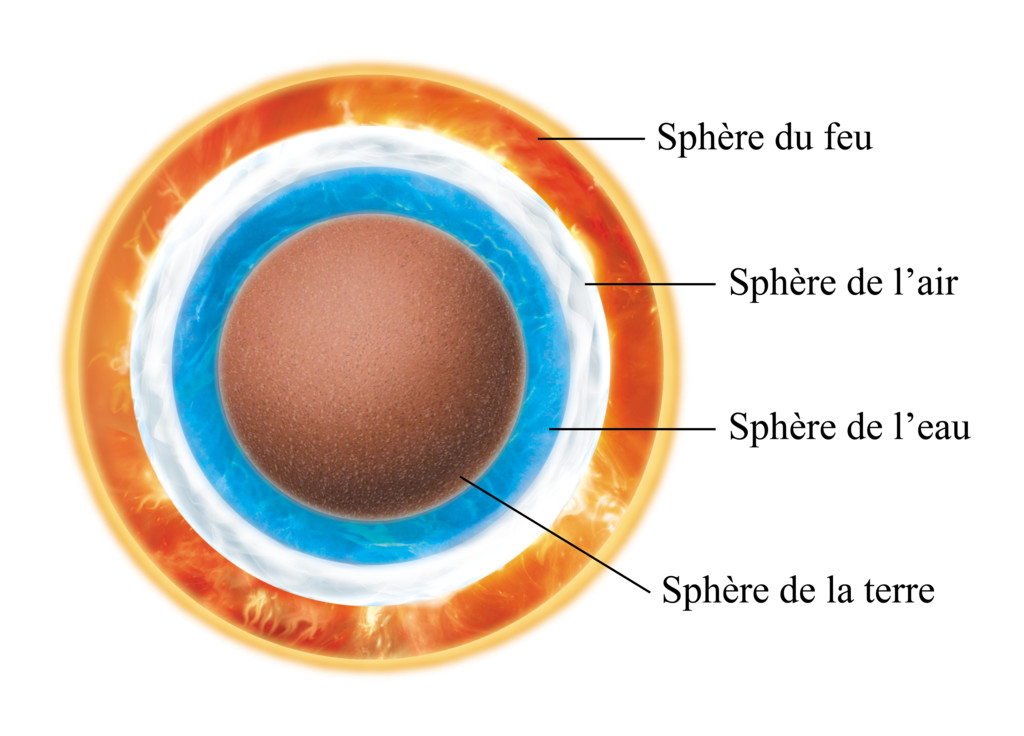
\includegraphics[scale=.8]{Sublunaire.jpg}
\centering
\caption{Monde sublunaire d'Aristote}
\end{figure}

Ainsi, chaque objet tendrait à rejoindre sa sphère d'origine : un caillou lâché à tendance à chuter dans l'air et couler dans l'eau, tandis que le feu a tendance à s'envoler dans les airs lorsqu'il est formé.\\

Pour le monde supralunaire, chaque astre est sur une orbite circulaire autour de la Terre, ce que Ptolémée synthétisera.

\subsection{Premiers échecs}

Au long du Moyen-âge, les méthodes d'observation se sont améliorées, et on observe quelques écarts avec la théorie de Ptolémée, le saint cercle n'est plus et on observe des "rebroussements" de planètes qui ne sont pas prédites par Ptolémée et Aristote. Ptolémée expliquait ceci en considérant que les astres tournaient sur un "petit cercle" donc le centre se déplaçait en orbite circulaire autour de la Terre, expliquant ces rebroussements. On appelle ceci des épicycles. En imbriquant ces petits cercles et épicycles, les astronomes ont réussi à expliquer le mouvement des planètes (en enchaînant jusqu'à 20 épicycles parfois).

\begin{figure}[H]
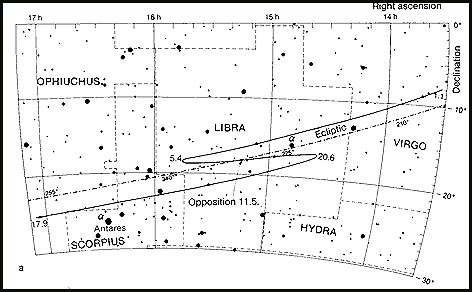
\includegraphics[scale=1.5]{Mars.jpg}
\centering
\caption{Mouvement apparent de Mars en 1984}
\end{figure}

Vers la fin du 16ème siècle, beaucoup de gens commençaient à se demander si l'ajout toujours plus grand d'épicycles pour coller aux trajectoires réelles était cohérent, surtout depuis que George Peurbach montra que la trajectoire des planètes était celle (circulaire) des planètes autour du Soleil plus celle du Soleil (circulaire) autour de la Terre, en éliminant plein d'épicycles.\\

Copernic, séduit par cette théorie, essaye de développer ses conséquences, qu'on peut lister ci-dessous :
\begin{propositionfr}{Conséquences de l'héliocentrisme de Copernic}{}
\begin{itemize}
\item Simplification des trajectoire en évitant la multiplication des épicycles
\item Explication de difficultés à observer les étoiles : quand Vénus et Mercure ne sont observables qu'en début/fin de nuit, c'est car elles sont plus proches du Soleil.
\end{itemize}
\end{propositionfr}

Cette théorie a un grand avantage de pouvoir expliquer les mouvements du monde supralunaire de manière un peu plus simple, mais on ne sait pas comment prédire les trajectoires circulaires, et pourquoi elles le sont ?

\subsection{Travaux de Kepler}

Johannes Kepler, en se basant sur les travaux de Tycho Brahe, essaye d'expliquer les trajectoires du monde supralunaire. Tycho Brahe mettait un point d'honneur à rendre le plus précises ses mesures, qui se basent sur de la trigonométrie, et qui donnent une précision à $2$ minutes d'angle (ce qui correspond à un trentième de degré). Ces mesures de haute précisions permettront à Kepler d'observer ses 3 lois de Kepler se basant sur les ellipses, dont nous introduisons les caractéristiques à présent :

\begin{définition}{Ellipse et foyers}{}
	Une ellipse est définie par l'équation suivante :
	$$\left(\frac{x}{x_0}\right)^2 + \left(\frac{y}{y_0}\right)^2 = 1$$
	On définit les foyers $F$ et $F'$ d'une ellipse comme les deux points tels que pour tout point $M$ de l'ellipse, $FM + FM' = \textrm{cste}$
\end{définition}

\begin{définition}{Demi grand-axe}{}
	On appelle le demi grand-axe $a$ la moitié de la distance reliant les deux points les plus éloignés de l'ellipse.
\end{définition}

\begin{figure}[H]
\centering
\begin{tikzpicture}
  \draw (0, 0) ellipse (3cm and 2cm) {};
	% \draw [domaine={-3}{3}, samples=800] plot (\x, {2*sqrt(1-(\x/3)^2)});
	% \draw plot [domaine={-3}{3}, samples=800] (\x, {-2*sqrt(1-(\x/3)^2)});
	\draw[<->] (-3, 0) -- (0, 0);
	\draw (-1.5, 0) node[above]{$a$};
	\point{-2.236}{0}{$F$};
	\point{2.236}{0}{$F'$};
\end{tikzpicture}
\caption{Une ellipse}
\end{figure}

\begin{théorème}{Lois de Kepler}{}
	\begin{enumerate}
	\item Les trajectoires des planètes autour du Soleil sont des ellipses, dont le Soleil est un des foyers
	\item Les aires balayées par la planète autour du Soleil sont constantes
	\item La période de révolution $T$ autour du Soleil et le demi-grand axe $a$ sont reliés de la manière suivante : $\frac{T^2}{a^3} = \textrm{cste}$.
	\end{enumerate}
\end{théorème}

\begin{figure}[H]
\centering
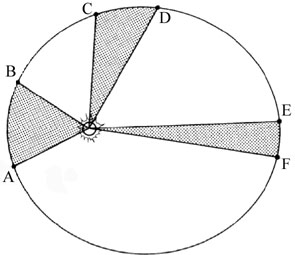
\includegraphics[scale=1.5]{2LDK.jpg}
\caption{Illustration de la deuxième loi de Kepler}
\end{figure}

On dit adieu aux cercles parfaits et on introduit les ellipses ! Cette vision plus l'héliocentrisme permettent d'avoir une bonne reproduction théorique des expériences, ce qui est assez bien (et novateur d'avoir pensé à ça).\\

Kepler commence à envisager qu'il existe une attirance mutuelle entre deux corps (tout comme les Marées qu'il explique par l'attraction de la Lune) mais pour lui les orbites des astres restent assez floues, à cause d'une "force immatérielle" qui lui reste assez difficile à comprendre.

\section{Réunification et gravitation classique}

Notre théorie actuellement est assez peu satisfaisante car elle distingue un monde sublunaire où la gravité est expliquée par Aritstote jusqu'ici et un monde supralunaire où Kepler fait émerger la forme des orbites sans comprendre réellement pourquoi. Nous allons voir comment on peut relier ces deux éléments.

\subsection{Galilée sur Terre...}

Pour Galilée, la chute des corps sur Terre semble assez étrange : on a une chute qui est assez différente en fonction des objets. Pour lui, cela vient de la résistance apportée par l'air, et il va essayer de s'en affranchir.\\

Pour cela, il va placer des boules "polies et lisses" sur des plans inclinés. L'observation sur des plans inclinés lui permet de s'affranchir des frottements de l'air, et les boules "polies et lisses" de s'affranchir de frottements avec le plan incliné (qui sont dûs à des irrégularités de structure). Avec un système de clochettes, il effectue un relevé de temps et de distances parcourues pour différentes masses.

\begin{figure}[H]
\centering
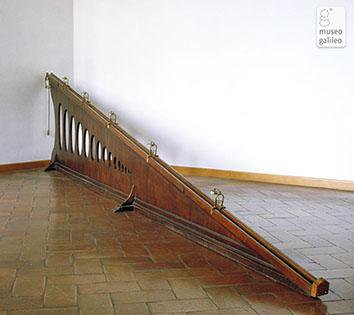
\includegraphics[scale=.7]{Clochettes.jpg}
\caption{Illustration de l'expérience de Galilée}
\end{figure}

\begin{propositionfr}{Observations de Galilée}{}
\begin{itemize}
\item Principe d'inertie : tout objet qui se déplace horizontalement ne voit pas sa vitesse modifiée.
\item On a l'universalité de la chute des corps : tous les corps chutent de la même manière, peu importe leur masse !
\item La distance parcourue varie comme le temps au carré, ce qui signifie que l'accélération (qui est la dérivée seconde de la position) est constante. On obtient que sur Terre les trajectoires de chute libre sont des paraboles.
\end{itemize}
\end{propositionfr}

Bon on a un présent un modèle plausible et un peu plus quantifié que celui d'Aristote, qui donne des résultats concluants pour l'étude des chutes sur Terre. Comment réunifier les deux points de vue supra/sublunaire ?

\subsection{Newton, mécanique et réunification}

Newton arrive à élaborer une loi qui est universelle (qui ne dépend pas d'une force supplémentaire comme l'entendait Kepler) réunifiant les deux théories de Kepler et Galilée. Avant de la développer, introduisons plusieurs notions :

\begin{définition}{Accélération}{}
L'accélération $\vec{a}$ est la dérivée de la vitesse mais aussi la dérivée seconde de la position.
\end{définition}

\begin{définition}{Force}{}
Une force décrit l'interaction d'un objet avec un autre. On la représente par un vecteur spécifiant le sens et la direction de l'interaction.
\end{définition}

\begin{définition}{Référentiel}{}
Un référentiel est un système d'axes et une horloge sur lesquels se sont mis d'accord des observateurs pour décrire de la même manière un mouvement.
\end{définition}

\begin{théorème}{Lois de Newton}{}
\begin{enumerate}
\item Tout corps qui n'est soumis à aucune force garde sa vitesse constante
\item On a $m_I\vec{a} = \vec{F}$ où $m_I$ est la masse dite "inertielle", $\vec{a}$ est l'accélération du corps et $\vec{F}$ et l'ensemble des forces qui s'exercent sur le corps dans certains référentiels dits galiléens.
\item Gravitation : Il existe une force gravitationnelle s'exerçant entre deux corps dirigée selon l'axe des deux corps dont la norme vaut
$F \sim m_{G1}m_{G2}f(d)$ où $m_G$ est la masse dite grave des deux corps et $f$ est une fonction de $d$ la distance entre les deux objets. La notation $a \sim b$ signifie qu'il y a relation de proportionnalité entre $a$ et $b$.
\end{enumerate}
\end{théorème}

\begin{théorème}{Transformation de Galilée}{}
Pour un référentiel $\mathcal{R}'$ se déplaceant à une vitesse $\vec{u}$ par rapport à un référentiel $\mathcal{R}$, la vitesse dans le référentiel $\mathcal{R}'$ vaut $\vec{u}$ plus celle dans le référentiel $\mathcal{R}$.
\end{théorème}

\begin{remarque}{Groupe de Galilée}{}
On a donc que tout référentiel qui se déplace à une vitesse constante par rapport à un référentiel galiléen est galiléen
\end{remarque}

Pour que cela vérifie Kepler, il faut (ce qu'on peut montrer avec les trois lois de Kepler) que $f(d) = \frac{1}{d^2}$, et Newton montre ainsi que $F$ vérifie les trois lois de Kepler ! Une bonne première étape.\\

Et sur Terre, ça donne quoi ? Quelque chose qui a été observé par Galilée est l'universalité de la chute des corps, qui permet donc de dire que $a_1 = a_2$ pour deux corps différents en chute libre. On a donc
$$F_1\sim \frac{m_{G1} m_{GT}}{R^2} \sim m_{I1}a_1$$
d'où sachant $a_1 = a_2$ on a $\frac{m_G}{m_I} = \textrm{cste}$.
Cette propriété est très intéressante car on a donc $m_G\sim m_I$ et en faisant un choix judicieux d'unités on a $m_G = m_I$ : on appelle ceci le principe d'équivalence faible.\\

Expérimentalement, cela fonctionne assez bien ! Par exemple, en remarquant des anomalies dans la trajectoire d'Uranus, Urbain le Verrier prédit l'existence d'un corps massif dont il prédit la position : Neptune est ainsi découverte !

C'est grâce à cette loi qu'est mesurée la masse de la Terre. Il nous manque cependant la constante de proportionnalité entre la force et le reste : elle est mesurée à l'aide d'une balance de torsion par Cavendish.

\begin{figure}[H]
\centering
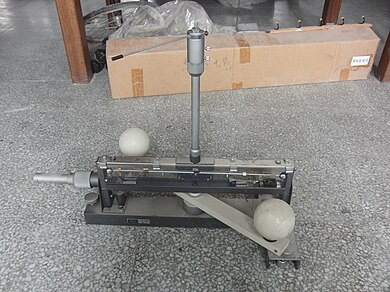
\includegraphics[scale=.7]{Cavendish.jpg}
\caption{Balance de torsion}
\end{figure}

\subsection{Encore des échecs ?}

Ici on se heurte à un nouveau problème : notre théorie n'est pas pleinement satisfaisante. Pour Newton, le problème des corps de masse nulle n'est pas réglé clairement, est ce qu'on a $\vec{a} = \vec{g}$ ou bien $\vec{a} = \vec{0}$ ? Dans le cas où $\vec{a} = \vec{g}$, Soldner prédit en 1801 que la lumière devrait être déviée de $0.875$ secondes d'angle avec son passage près du Soleil (à retenir pour plus tard), et on trouve un rayon d'un trou noir qui ne correspond pas à la vie réelle.\\

Dans la théorie Newtonienne, la trajectoire de Mercure serait une ellipse dont le périhélie (le point le plus proche du Soleil de l'ellipse) bouge à une vitesse de $531$ secondes d'arc par siècle. En réalité, observe que le périhélie se déplace à $575$ secondes d'arc par siècle (fun fact : Urbain le Verrier, voyant des planètes partout, a encore postulé l'existence d'une nouvelle planète "Vulcain" qui n'existe en réalité pas).\\

Notre théorie n'est pas parfaite, et on va devoir sortir l'artillerie lourde pour trouver des solutions.

\section{Relativi-thé}

\subsection{Relativité restreinte}

Peu après la mécanique Newtonienne naît l'électromagnétisme. Maxwell fait émerger via ses équations une vitesse $c$ significative : la vitesse de la lumière dans le vide. Le problème cependant est que la théorie Galiléenne ne fait pas apparaître de vitesse limite, et qu'il n'est pas possible de donner une utilité à $c$ dedans : Einstein (avec l'aide d'autres comme Lorentz) va essayer de concilier Électromagnétisme et Mécanique Galiléenne : l'électromagnétisme étant très bien vérifié expérimentalement, la mécanique galiléenne semble être la coupable.

On introduit une transformation différente des vitesses, ce qui amène à la constance de la vitesse de la lumière dans tous les référentiels, la dilatation du temps et d'autres phénomènes.

\subsection{Relativité générale ?}

Nous avons réconcilié Mécanique Galiléenne et Électromagnétisme, mais à présent notre gravité ne correspond plus. Le concept même de force pose de gros problèmes à Einstein qui essaye d'unifier les deux théories avec la gravitation. Pour cela, il fait l'expérience de pensée suivante : en mettant un observateur en chute libre dans un ascenseur en chute libre, c'est équivalent à un observateur qui serait immobile dans un référentiel immobile. Ainsi, il aboutit au principe dit d'Einstein : les expériences de mécanique sont identiques dans un référentiel accéléré avec gravité ou bien dans un référentiel immobile sans gravité.\\

Plus loin, il affirme même le principe d'équivalence forte : toute expérience en général est identique dans un référentiel accéléré avec gravité ou bien dans un référentiel immobile sans gravité.\\

Ok très bien cette expérience de pensée étant faite, on peut se demander si il existe un changement de coordonnées affines pour passer d'un référentiel avec gravité à un référentiel sans gravité : la réponse est non. Par exemple sur Terre, on peut considérer le référentiel qui est en chute libre par rapport à un point $A$. En revanche, pour un point $B$ différent, dans ce référentiel la gravité n'est pas nulle car sinon on aurait que les directions des accélérations seraient les mêmes ce qui est faux par exemple pour la Terre qui est courbée.\\

On a donc besoin d'un changement de coordonnées courbe qui fasse apparaître ce phénomène : la courbure de l'espace temps est née. Qu'est ce qui cause cette courbure ? On peut voir que c'est l'énergie qui crée la courbure, et que la courbure de l'espace-temps peut être reliée au contenu de l'univers grâce à l'Équation d'Einstein.

\section{Et maintenant ?}

Un problème ne reste pas encore réglé : c'est celui de la vitesse de rotation des galaxies : le modèle Newtonien prévoit la courbe en pointillés tandis que la réalité donne quelque chose comme la courbe rouge.

\begin{figure}[H]
\centering
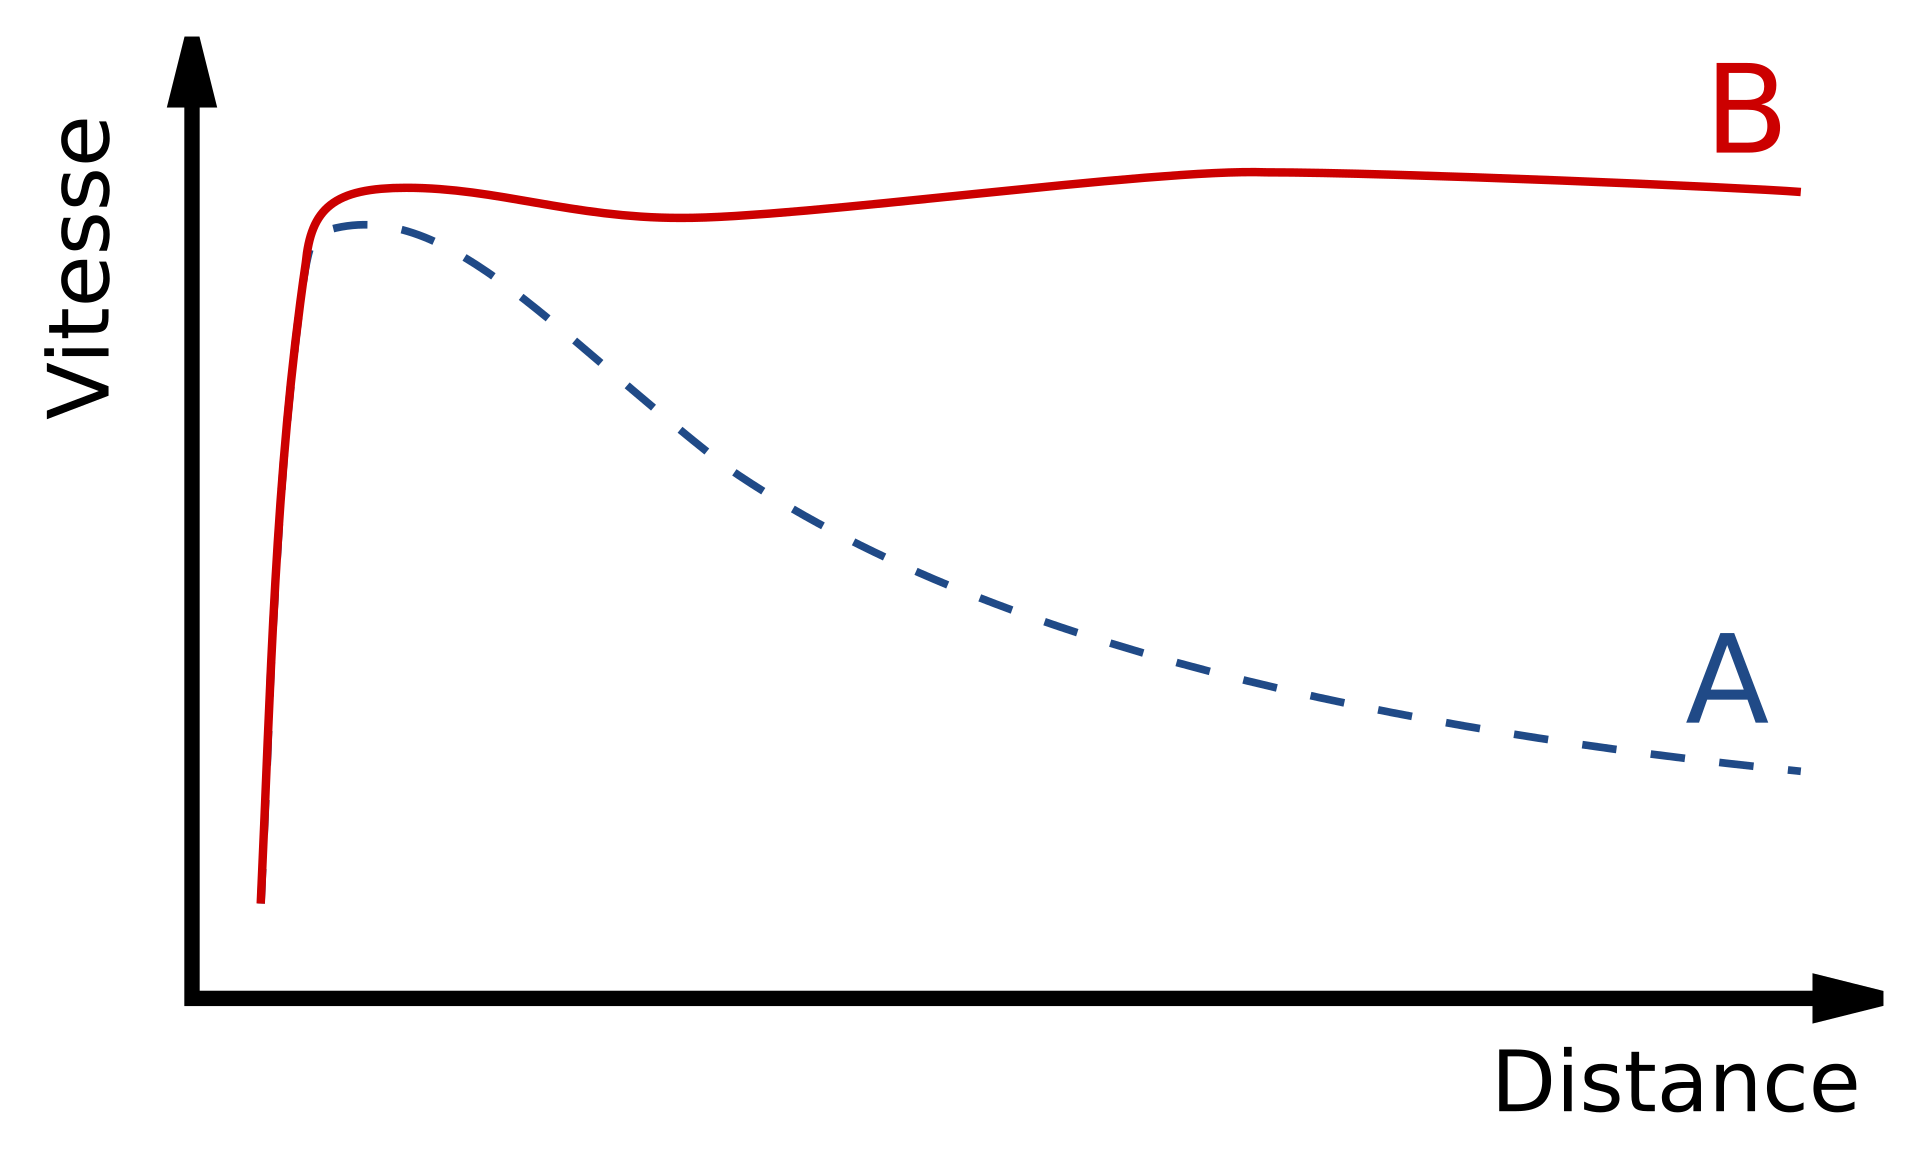
\includegraphics[scale=.16]{MatNoire.png}
\caption{Vitesse de rotation en fonction du rayon}
\end{figure}

Un nouveau problème qui serait à l'origine à soit de réflexions sur la théorie actuelle, ou bien l'introduction d'une "matière noire". Tant de questions qu'il reste à éclaircir, et l'impression d'être revenus à l'époque d'Aristote où nous avons une théorie qui fonctionne assez bien, pour \textit{presque tout}.

\end{document}
